% CREATED BY DAVID FRISK, 2015
\chapter{Introduction}
\lettrine[findent=2pt]{\fbox{\textbf{T}}}{ }he thesis presents the study of automated visualization of the electrical system of Volvo Car Group company using the identified artifacts from a set of data of the system's database. The artifacts are derived from analysing the needs of different stakeholders. The thesis also reports an evaluation of the provided automated visualization to the way of working with Electrical Power System (EPS) and in the electrical department of the company.

\section{Background}\label{Background_ref}
One of the biggest challenges in automotive industry during the past few years is to build vehicles that meet customer expectations. To overcome the challenge, more complex system of mechanical and electrical components are designed and built in modern vehicles. Besides that, a huge number of software is also integrated in order to carry out certain tasks, resulting in up to 70 of Electrical Control Unit (ECUs) deployed in a car \cite{Beeck}. For this reason, creating the architecture of the complex system is of importance to ensure that every components and the communication among them are in the right places. \\

Volvo Car Group is a Swedish premium automotive manufacturer producing modern vehicles to the world. At the company, two types of architectures for electrical system are used to handle complex systems of cars \cite{Eliasson_1}. The two architectures have different abstract levels, meaning that they serve different purposes. A high-level architecture (logical view) contains Logical Architectural Components (LAC) designed by software architects with a purpose of guiding and breakdown work to be developed during implementation phase. Development team creates a low-level architecture (design view) which represents actual structure of the electrical system. The low-level architecture also shows Logical Components (LC) which are broken down from LACs in the high-level architecture, it also shows communication between LCs, and signals they receive/send. \\

The low-level architecture is stored in a proprietary tool called \textit{Elektra} which is database that stores the data such as documentations, the software components, the ECUs, the LCs, and the LACs. Using the stored data, the tool generates model shells to be implemented by software developers for in-house software development and also the tool generates requirement documents which has functionalities to be implemented by suppliers. Moreover, it can also generate ECU-integration and network communication in the electrical system \cite{Eliasson_2}.\\

When a user interacts with \textit{Elektra}, he/she will be presented with a complete view of the whole low-level architecture of an electrical system. The tool does not allow users to select and generate visualization of some parts of the system. The architecture is enormous since it contains all LC and their communication, making them difficult for both teams and other stakeholders to see. Thus, visualization of the low-level architecture is needed. To do so, an identification of the key components of electrical system must be performed since visualizing the whole architecture is unnecessary for all stakeholder. \\

\begin{figure}[H]
\centering
\captionsetup{justification=centering}
\vspace{0cm}% Adjust vertical spacing here
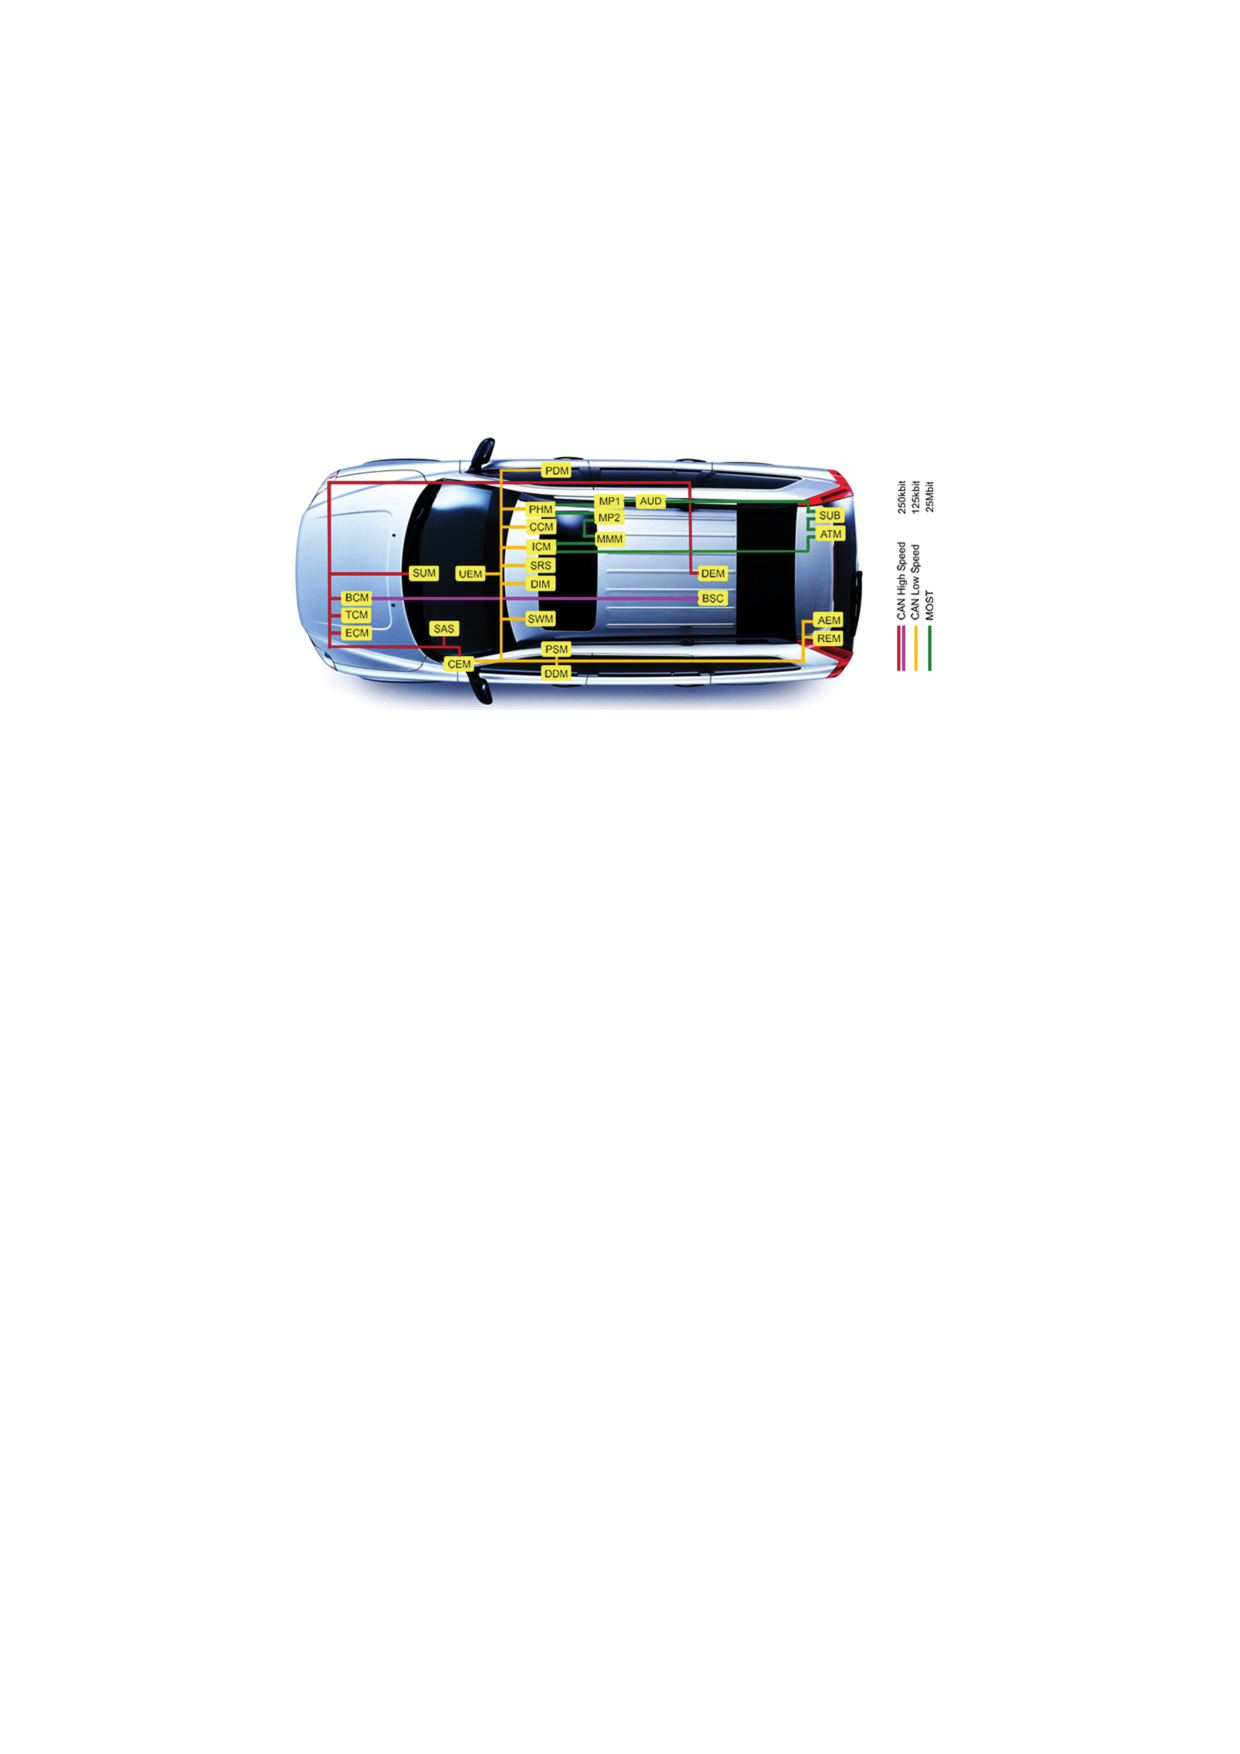
\includegraphics[width=0.9\linewidth]{figure/literatures/wallin_physical.pdf}
\caption{An example of electrical architecture of the Volvo XC90~\cite{Wallin}}
\end{figure}

Apart from what has been mentioned, inconsistency between the high- and the low-level architectures arises. The reason is that the low-level architecture is kept up-to-date by the development team during the implementation phase as the product evolves, but the high-level one is updated only a few times per year. Having a visualization of the low-level architecture may helps to bridge the gap of inconsistency between both levels of the architectures.


\section{Statement of the problem} \label{Statement_ref}
The first problem that this thesis work addresses is, \textit{Elektra} shows the irrelevant parts of the system to its users. This means, it shows the complete view which includes all components, ports, and their interactions between them. Moreover, the tool does not provide a visualization. In most cases, only some parts of the data stored in \textit{Elektra} are relevant to the stakeholders. This depends on the  individual’s interest. Due to this, it is difficult for stakeholders to locate what they are looking for unless they know where to look for it. Sometimes, the stakeholders do not even know what they are looking for and this makes a task to locate what they want even more difficult.

Furthermore, the diagram at VCG does not only contain the components, ports, and connections, but also a logical designs. This makes the document even bigger and harder for stakeholders to focus on only the parts that they have an interest in. \\ 

The second problem is, the inconsistency between the low-level and high-level architectures. Usually, the stakeholders who interact with the system may have certain features that are required to be implemented in the system. When the developers implement these features in a system, they are also required to update the low-level architecture regularly. So, this is the point where the inconsistency occurs. 

To tackle these two problems, our thesis will provide a solution which helps to create automated visualization of the current status of \textit{Elektra} with regard to the main interests of different stakeholders, also the solution will help high-level architects to get better understanding of what is going on in the real implementation which can support a decision making.


\section{Purpose} \label{Purpose_ref}
The purpose of this thesis work is to find metrics that helps to identify the key components of the electrical architectures. The metrics found are used as inputs to a visualization tool in order to create the visualization of the key components of the electrical architectures. The thesis also aims to find possible views (visualizations) of the electrical architectures with regards to the interests of different stakeholders. \\

Similar work has been done but the case was with class diagrams which is a bit different since \textit{Elektra} has logical components instead of classes \cite{}.

\section{Research questions} \label{RQ_ref}
In order to address the problem mentioned, we have 5 research questions. The research questions covers the identification of needs of stakeholders, their differences, complementing \textit{Elektra} and also the benefits of having the automated visualization of data stored in \textit{Elektra}. These are formulated as follows:

\begin{que} \label{que:1}
What are the needs of stakeholders towards the visualization of the architectural diagrams?
\end{que}

\begin{que} \label{que:2}
What are the differences of the needs from each stakeholder?
\end{que}

\begin{que} \label{que:3}
How do we identify the needs of stakeholders and come up with software metrics that can help to identify important components in the architectural diagrams?
\end{que}

\begin{que}\label{que:4}
How do we complement Elektra with a visualization tool?
\end{que}

\begin{que} \label{que:5}
How does the automated visualization of the architectural diagrams impact the way of working?
\end{que}


\section{Limitation} \label{Limitation_ref}
The first procedure that was followed was to conduct interview sessions with different stakeholders at Volvo Car Group and to find out what the important components that they want to see in the electrical architectures were. However, there are some limitation to the work at the time of the study. Firstly, only a small group consisting of two stakeholders was selected to participate in identifying the key components due to time limitation which made it impossible to involve all stakeholders. \\

Secondly, the visualization tool that was used together with the metrics that were discovered from the stakeholders might be specific and perhaps the results of the visualization could not be the same if any other different tool was used. \\

Lastly, the visualization that was achieved using the metrics might not be applicable to other groups of stakeholders, or in other companies. The thesis work is performed at Volvo Car Group and hence the metrics that were discovered might only be applicable in the company or similar company where the same way of modelling electrical architectures is created.


\section{Outline of the report} \label{Outline_ref}
This report is divided into 6 chapters which can be seen in . 
\begin{figure}[H]
\centering
\captionsetup{justification=centering}
\vspace{0cm}% Adjust vertical spacing here
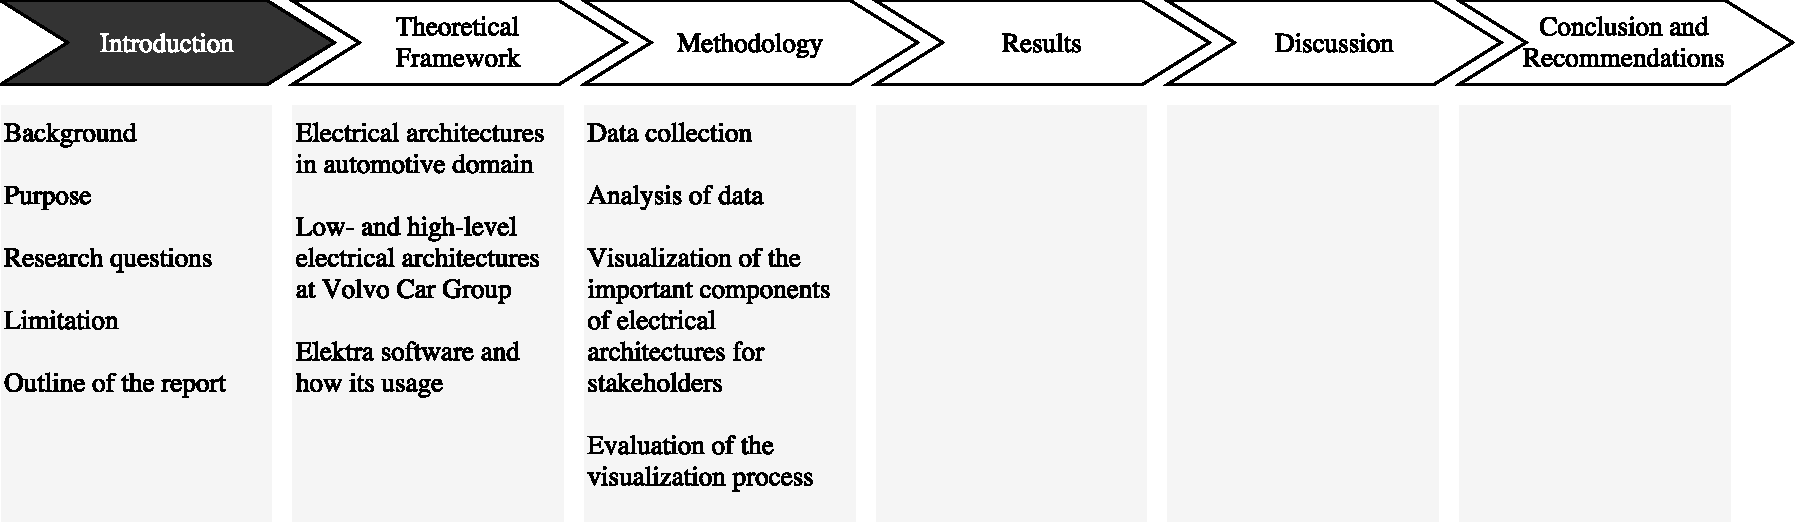
\includegraphics[width=1\linewidth]{figure/report_outline.pdf}
\caption{Report outline}
\end{figure}